
\section{Modeling of the \Fermi bubbles at low latitudes}

One of the main problems in the analysis of the FB near the GC is the 
presence of the foreground emission components, 
such as the interactions of cosmic rays with the interstellar gas and radiation fields.
In order to test the possible effects of the foreground emission modeling,
we use several methods to estimate the contribution of the foreground emission to the data.

In particular, there is a tentative
displacement of the FB to the right of the GC, e.g., negative Galactic latitudes \citep{2016ApJS..223...26A, 2017ApJ...840...43A},
with a spectrum that is harder than the spectrum of the FB at high latitudes \citep{2017ApJ...840...43A}.
If we assume that the Galactic emission components are approximately symmetric with respect to the GC,
then we can simply mask PS and calculate the difference in gamma-ray flux to the left and to the right from the GC.
The difference should be approximately equal to the asymmetric part of the FB emission
under the assumption that the other Galactic components and unresolved PS are symmetric with respect to the GC
(Section \ref{sec:data_diff}).

In order to further test the hypothesis of the asymmetric and hard emission from the FB at low latitudes,
we use the data at energies $\lesssim \SI{1}{GeV}$ to create a template of the Galactic emission,
provided that the expected contribution of the FB at these energies is small relative to the rest of the Galactic components.
Then we fit the template derived from the low energy data together with an isotropic template at higher energies
outside of the FB area.
The FB intensity is determined by extrapolating the model inside the FB area using the full template and by subtracting the model
from the data (Section \ref{sec:le_data_model}).
As an alternative approach, instead of fitting outside of the FB area, we add independent flat rectangular templates with the size
approximately following the FB size to the model and fit over the whole sky.
The flux attributed to these rectangular templates is used as an estimate of the average flux in the FB in the corresponding areas
(Section \ref{sec:box_model}).

We also calculate the flux attributed to the bubbles using one of the diffuse emission models from \citep{2017ApJ...840...43A}
(Section \ref{sec:galprop_model}).



\subsection{Left-right difference in the data}
\label{sec:data_diff}

As a first simple check of the assymmetry at low latitudes, we compare the unprocessed \Fermi-LAT data east and west of the Galactic center. After masking PS, we average the data over a region west, i.e. longitudes $\ell \in (-10^\circ, 0^\circ)$, and east, i.e. $\ell \in (-10^\circ, 0^\circ)$, of the Galactic center for different latitudes. The regions have a width of $10^\circ$ in latitude for high latitudes, $b >|10^\circ|$, and $4^\circ$ for low latitudes, $b <|10^\circ|$. The difference of the averaged diffuse emission west $-$ east is shown in Fig. \ref{fig:data_diff} as a function of energy. At high latitudes, $b >|10^\circ|$, the emission is very symmetric. The emission for latitudes $b \in (-6^\circ, -2^\circ)$ and $b \in (-2^\circ, 2^\circ)$ shows excessive emission west of the Galactic center, which does not decay for high energies. 


\begin{figure}[h]
 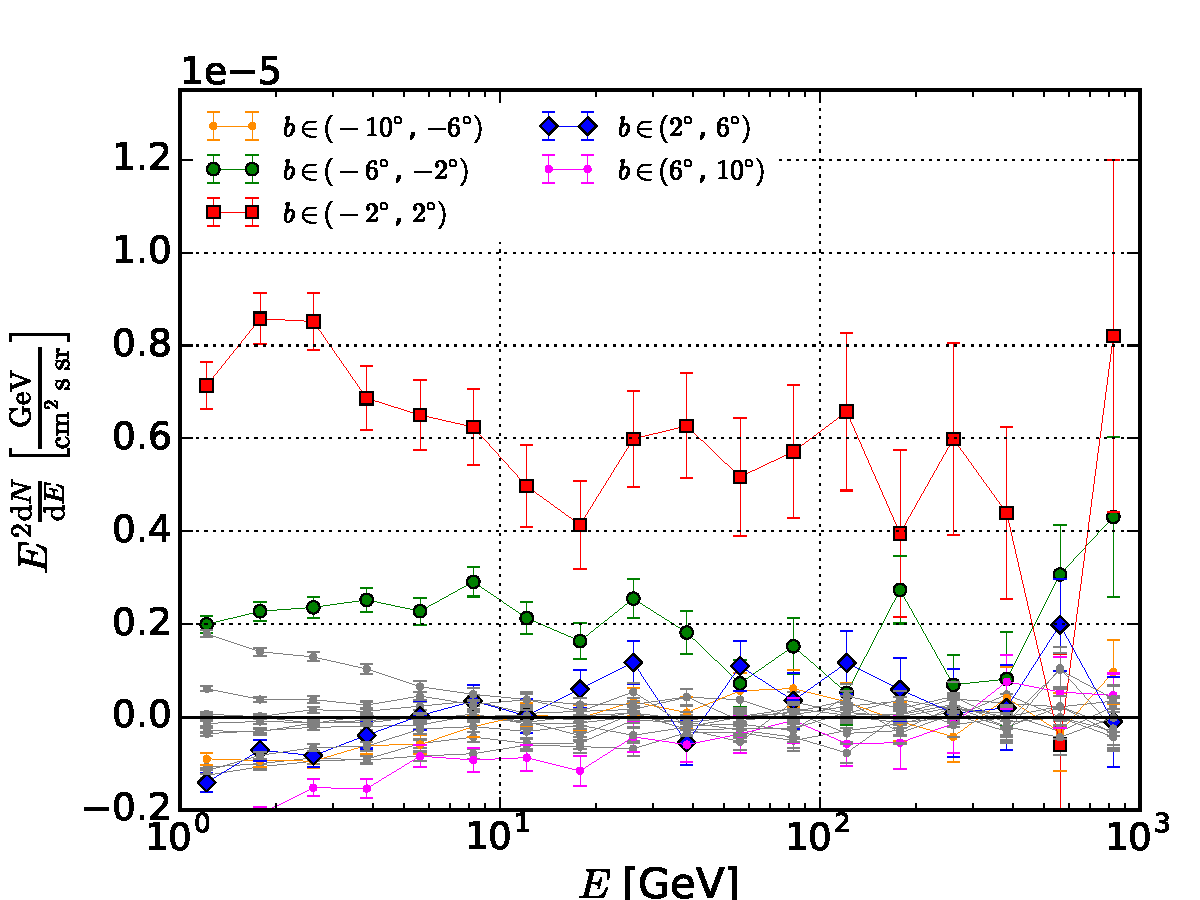
\includegraphics[width=0.5\textwidth]{plots/Difference_data_for_different_latitudes.pdf}
 \caption{Difference west $-$ east in the unprocessed \Fermi-LAT data with symmetric PS mask. The region west reaches from $-10^\circ$ to $0^\circ$ longitude, the region east from $0^\circ$ to $10^\circ$ longitude.}
 \label{fig:data_diff}
\end{figure}

\subsection{Low energy data as a background model}
\label{sec:le_data_model}

\begin{figure*}[t]
	\makebox[\textwidth][c]{
    	\begin{subfigure}{0.3\textwidth}
        	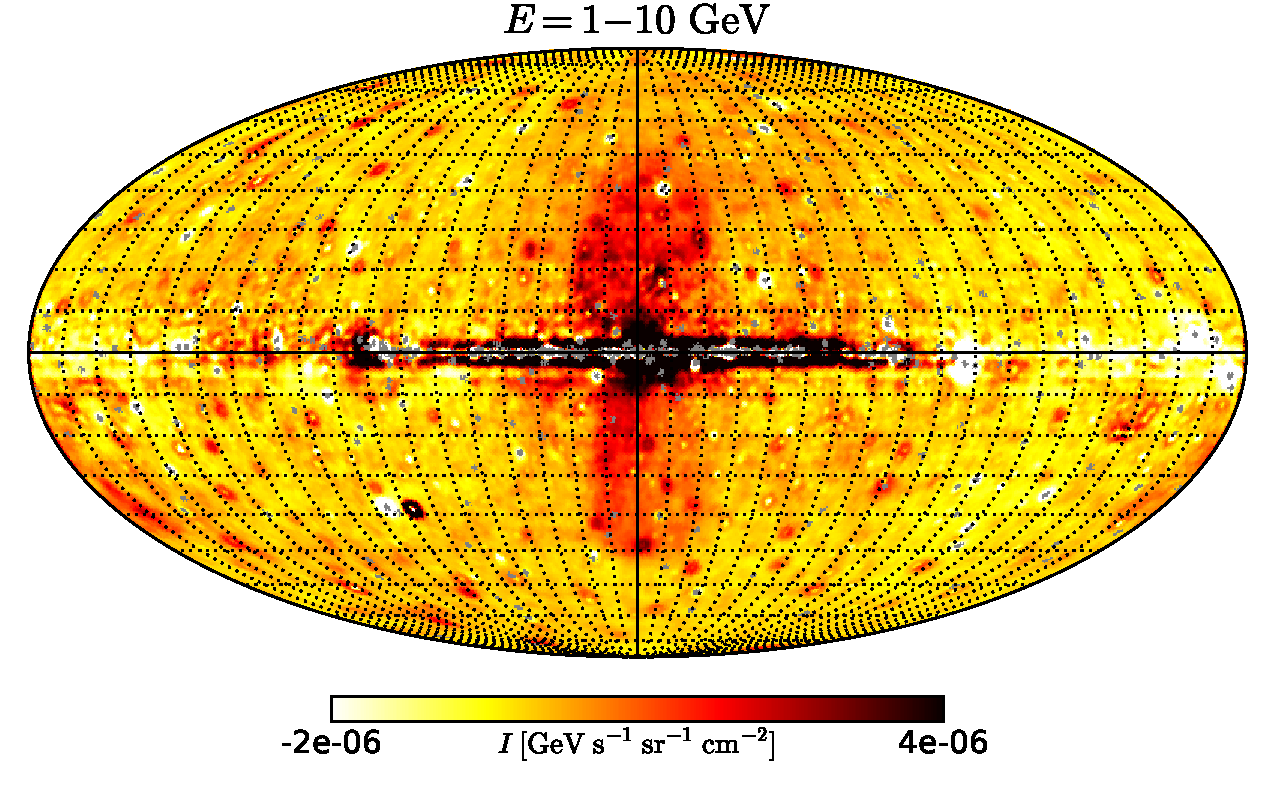
\includegraphics[width=\textwidth]{plots/Mollweide_LowE_03-10GeV_flux_source_range_0.pdf}
    	\end{subfigure} 
    	\begin{subfigure}{0.3\textwidth}
        	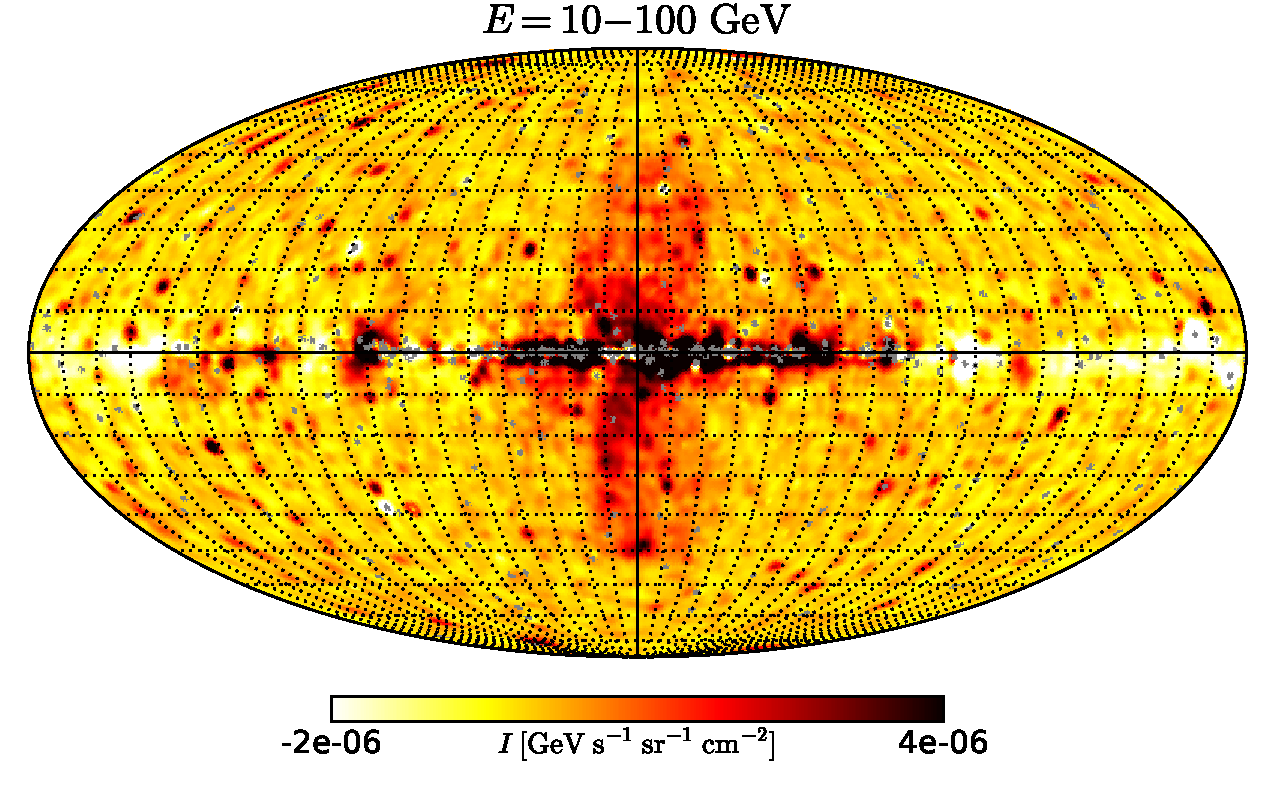
\includegraphics[width=\textwidth]{plots/Mollweide_LowE_03-10GeV_flux_source_range_1.pdf}
    	\end{subfigure}
    	\begin{subfigure}{0.3\textwidth}
        	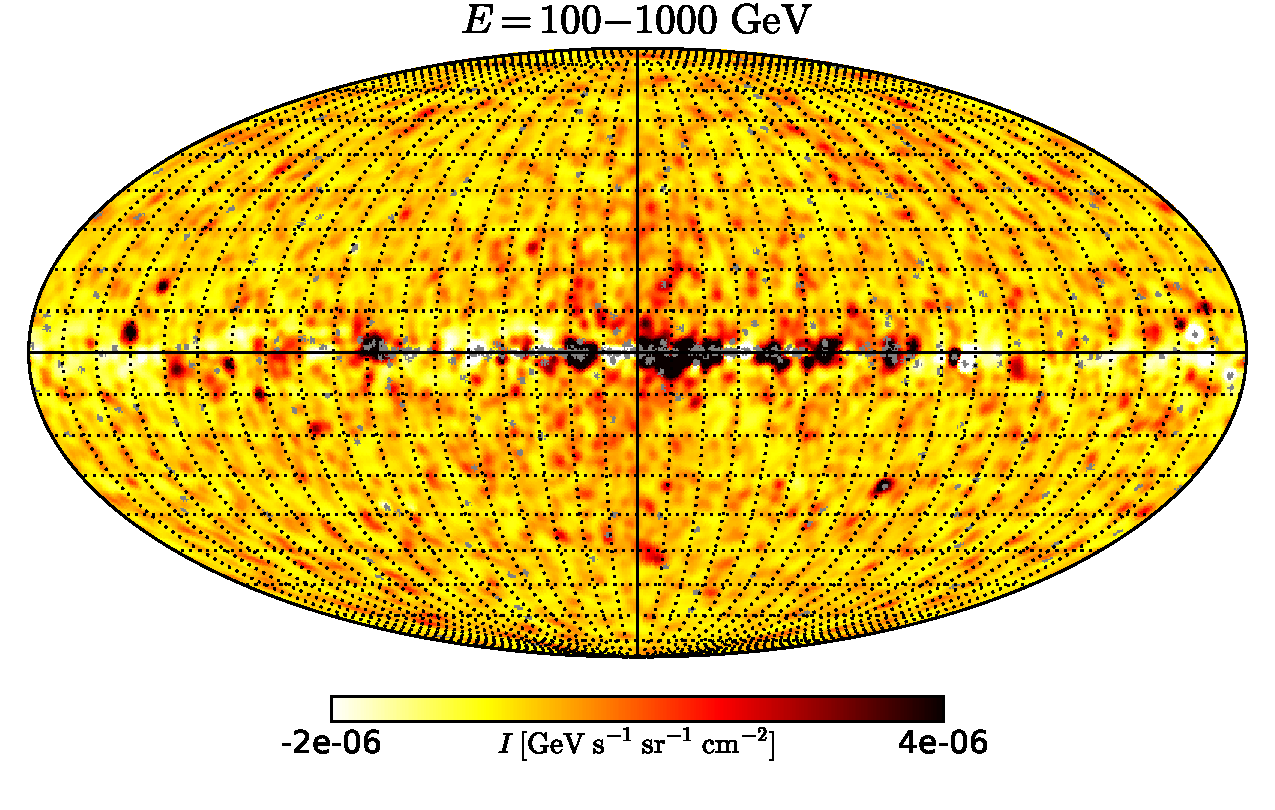
\includegraphics[width=\textwidth]{plots/Mollweide_LowE_03-10GeV_flux_source_range_2.pdf}
    	\end{subfigure}
    }
  	\caption{Residuals of the low-energy model for three different energy ranges. The \Fermi bubbles are clearly visible in the first two energy ranges. Point sources are masked.}
  	\label{fig:Maps_lowE}
\end{figure*}

Gamma rays produced in interactions of CR with gas and IC scattering dominate the gamma-ray emission around the GC in the energy range $E \lesssim \SI{1}{GeV}$. 
Consequently, low-energy \Fermi-LAT data is a good tracer for diffuse gamma-ray emission in the Galactic plane and can be used to create a spatial template for the Galactic foreground.
Since the angular resolution is worse for smaller energies, we smooth the data in each high-energy bin with a Gaussian kernel of $1^\circ$ to compensate for the difference in angular resolution. 

We cut the sky horizontally in latitude stripes with the width of $4^\circ$ and define our model in each stripe and energy bin separately. 
In the latitude stripe $\ell$ and energy bin $E$ our model consists of a term proportional to the low-energy photon counts $k_{\ell\alpha} \cdot \tilde N^\low_\ell(E,x)$, summed over all energies in 0.3 - $\SI{1.0}{GeV}$, and an additional term $\tilde c_{\ell}(E,x)$: 
\be
N^\model_{\ell}(E,x) = k_{\ell}(E) \cdot \tilde N^\low_{\ell}(E,x) +\tilde c_{\ell}(E,x).
\ee
The term $\tilde c_\ell(E,x)$ consists of a factor $c_\ell(E)$, which is constant in each latitude $\ell$ and energy $E$, that is weighted by the exposure $\tau(E,x)$:
\be
\tilde c_\ell(E,x) = c_\ell(E) \cdot \tau(x,E).
\ee
It takes into account the isotropic extragalactic background and partially compensates for the latitude dependent IC emission. To include the dependence of exposure on energy and positon in the sky, the low-energy data is weighted by the quotient of exposure $\tau(E,x)$ in the low- and high-energy range in each pixel $x$:
\be
\tilde N^\model_\ell(E,x) = \frac{1}{n_\low} \left(\sum_{\epsilon \in (0.3 - \SI{1.0}{GeV})} \frac{N^\low(\epsilon, x)}{\tau(\epsilon,x)}\right) \cdot \tau(E,x),
\ee
where $n_\low$ is the number of low-energy bins. 


We determine the parameters $c_{\ell}(E)$ and $k_{\ell}(E)$ by fitting the model to the \Fermi-LAT data in energy bins $E > \SI{1.0}{GeV}$
using Poisson likelihood (with Python iminuit minimizer). Since we smooth the data before the fit, the Poisson log-likelihood is an approximation in this case. To avoid an overcompensation of the \Fermi bubbles the region $-20^\circ < \ell < 20^\circ$ is excluded from the fit. 
We mask the 200 brightest 3FGL PS  with a circle of radius $\frac{\delta}{\sqrt{2}} + 1^\circ$ where $\delta = 0\degr\!\!.46$ is the characteristic size of the pixels. 
We also symmetrize the PS relative to the GC in order to avoid possible bias by masking more pixels on one side of the GC.

After we fit the model in each latitude stripe, we interpolate it inside the bubbles ROI and find the residual by subtracting it from the data.
Figure \ref{fig:Maps_lowE} shows the residual maps for three different energy ranges. 
The FB are clearly visible in the first two energy ranges, $E = 1 - \SI{10}{GeV}$ and $E = 10 - \SI{100}{GeV}$, for 
$E = \SI{100}{GeV} - \SI{1}{TeV}$ the statistics is low, but one can still see an excess near the GP.

\subsection{Rectangles model of the bubbles}
\label{sec:box_model}

Our first simple ansatz for a model of the FB consists of rectangular templates that approximately cover the area of the FB. As a model for the foreground we again use the low-energy model from Section \ref{sec:le_data_model}. As before, the fit is performed independently in each $4^\circ$ latitude stripe. To explore the east-west assymetry of the FB, two rectangular templates, one east ($-20^\circ - 0^\circ$) and one west ($0^\circ - 20^\circ$), are added to the low-energy model in each latitude stripe $\ell$ and energy bin $E$: 
\be
\begin{split}
N^\model_{\ell}(E,x) &= k_{\ell}(E) \cdot \tilde N^\low_{\ell}(E,x) +\tilde c_{\ell}(E,x)\\
&\quad + R^\east_\ell(E) + R^\west_\ell(E).
\end{split}
\ee
We determine the normalization of the rectangles $R^\east_\ell(E)$ and $R^\west_\ell(E)$ and the parameters $k_{\ell}(E)$ and $c_{\ell}(E)$ by fitting the model to the \Fermi-LAT data in energy bins $E > \SI{1.0}{GeV}$. The resulting residual, shown in Fig. \ref{fig:Maps_Rectangles} for $E = 10 - \SI{100}{GeV}$, is very similar to the low-energy model.

\begin{figure}[h]
 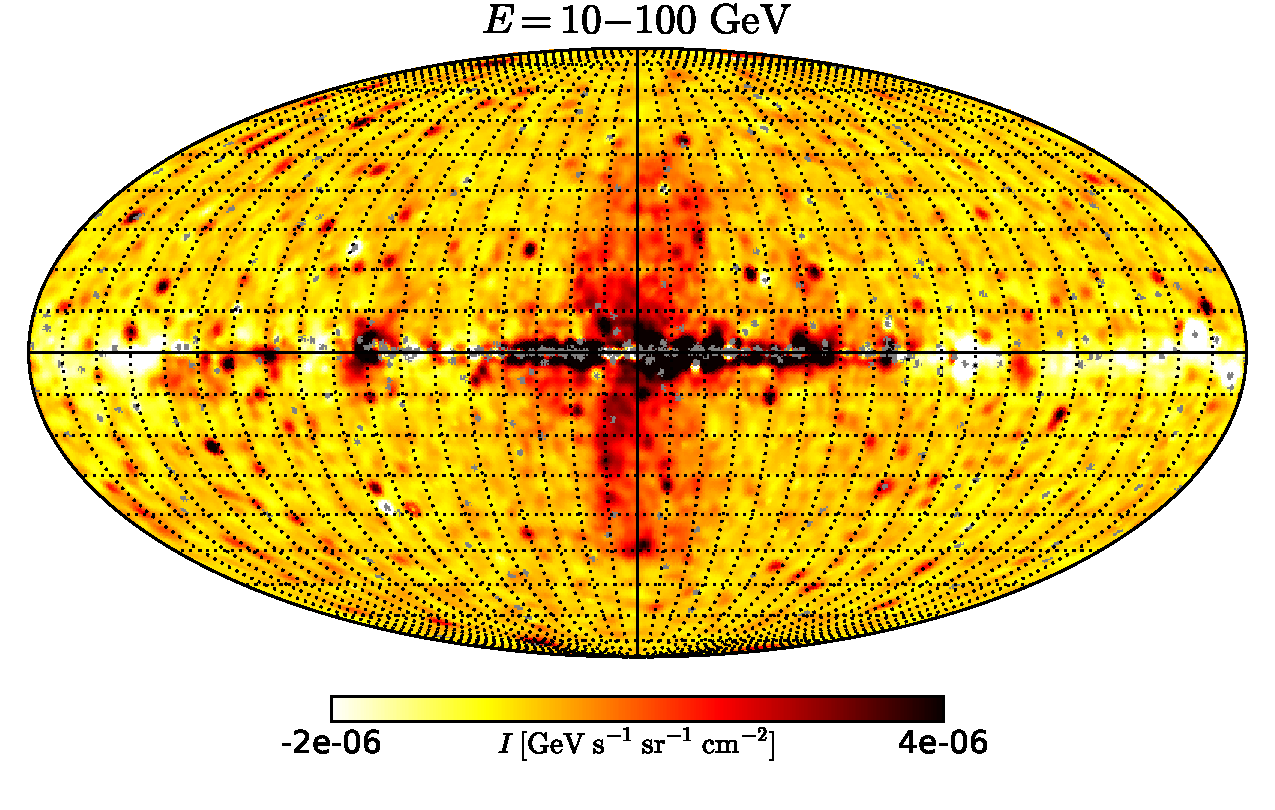
\includegraphics[width=0.5\textwidth]{plots/Mollweide_Boxes_residual+boxes_03-10GeV_flux_source_range_1.pdf}
 \caption{Rectangles-model residual.}
 \label{fig:Maps_Rectangles}
\end{figure}
%
%\begin{figure*}
%	\makebox[\textwidth][c]{
%    	\begin{subfigure}{0.3\textwidth}
%        	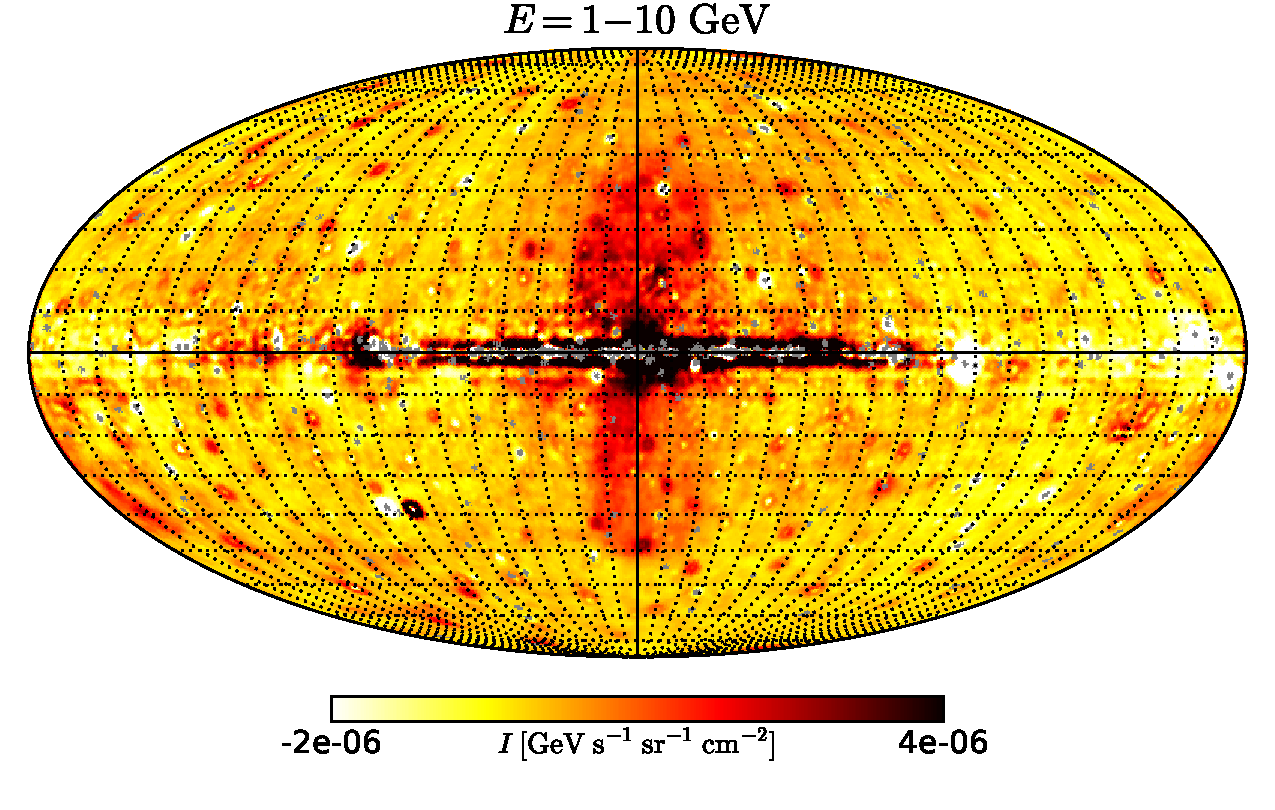
\includegraphics[width=\textwidth]{plots/Mollweide_Boxes_residual+boxes_03-10GeV_flux_source_range_0.pdf}
%    	\end{subfigure} 
%    	\begin{subfigure}{0.3\textwidth}
%        	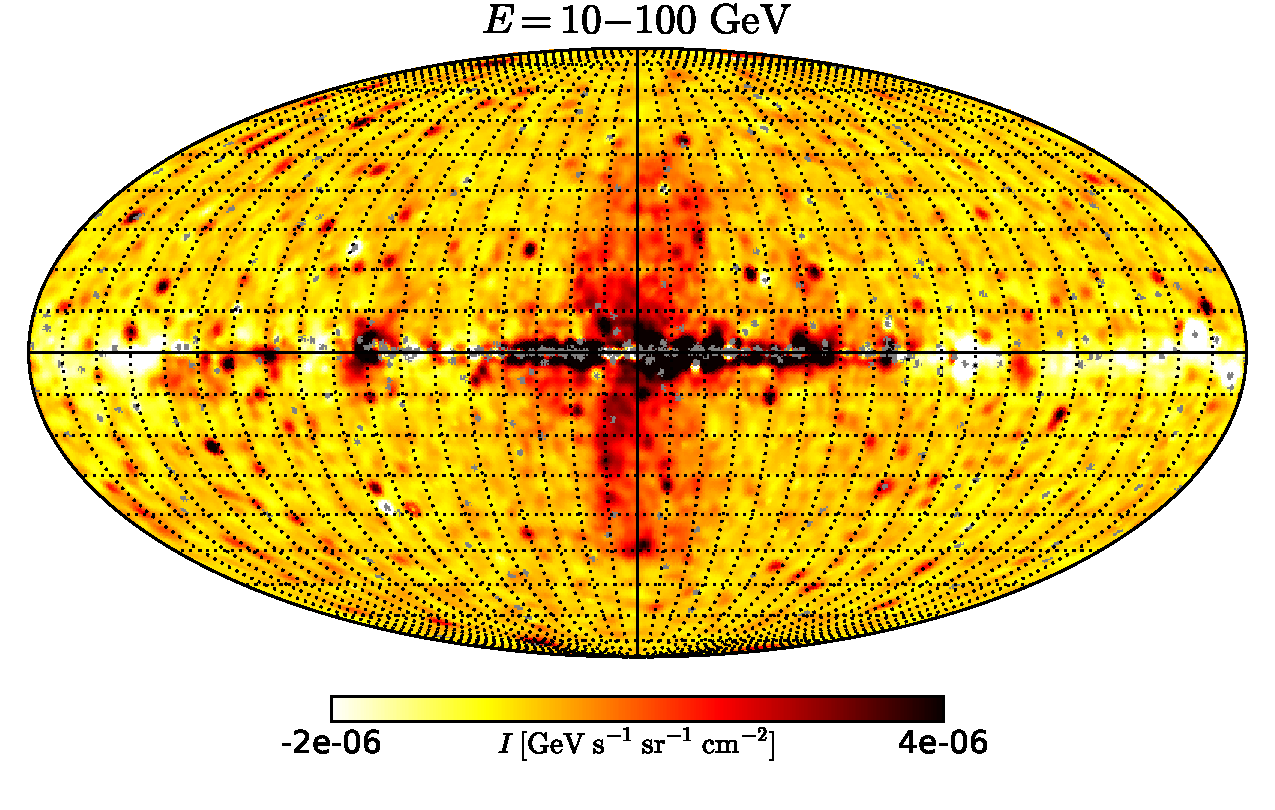
\includegraphics[width=\textwidth]{plots/Mollweide_Boxes_residual+boxes_03-10GeV_flux_source_range_1.pdf}
%    	\end{subfigure}
%    	\begin{subfigure}{0.3\textwidth}
%        	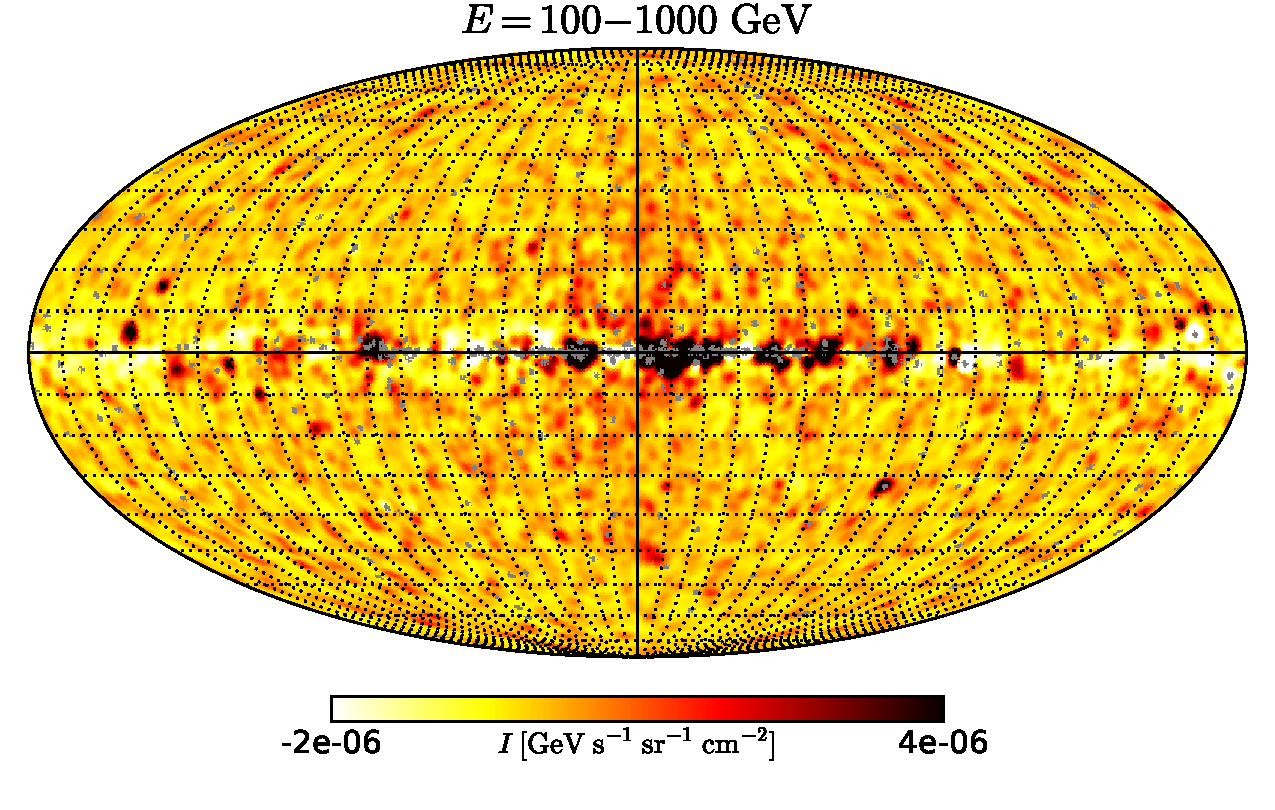
\includegraphics[width=\textwidth]{plots/Mollweide_Boxes_residual+boxes_03-10GeV_flux_source_range_2.pdf}
%    	\end{subfigure}
%    	}
%  	\caption{Rectangles-model residuals in three different energy ranges.}
%  	\label{fig:Maps_Rectangles}
% \end{figure*}
%

\subsection{GALPROP model of the foreground and PS refitting}
\label{sec:galprop_model}


\begin{figure}[h]
 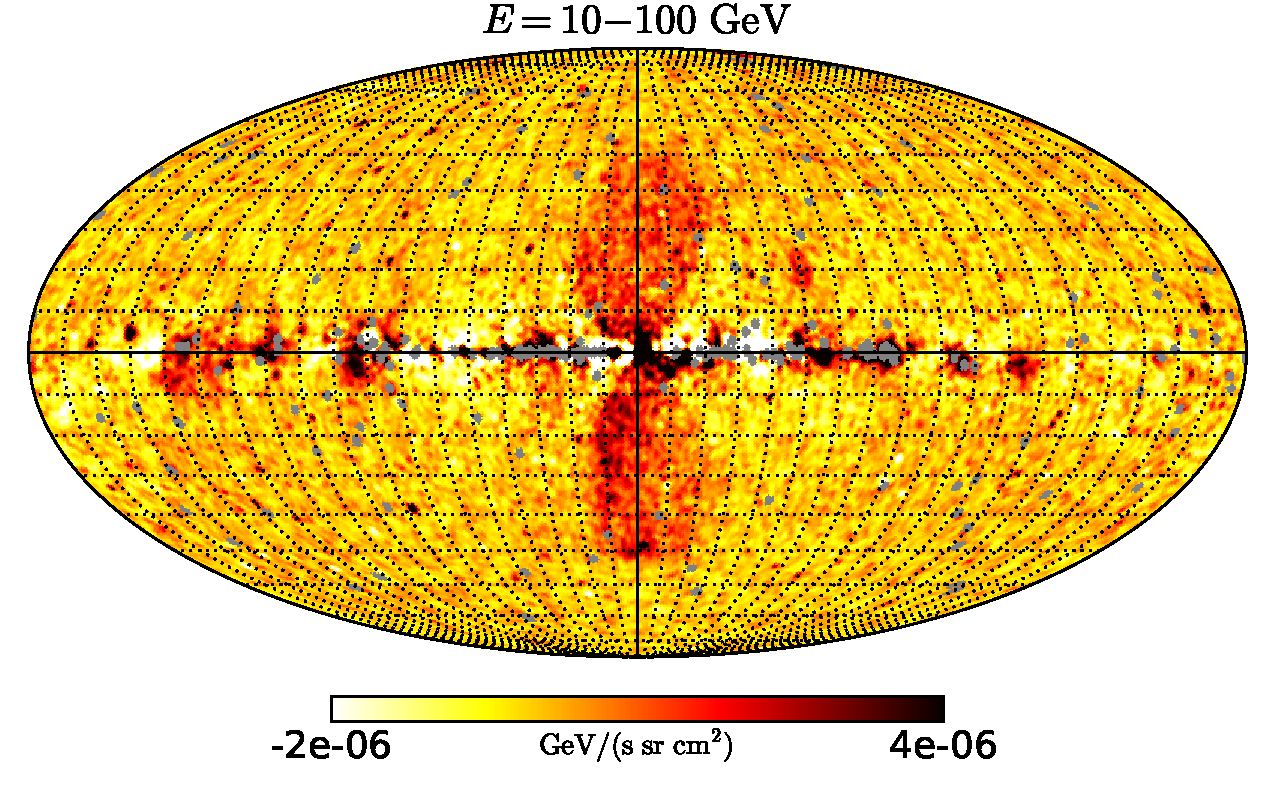
\includegraphics[width=0.5\textwidth]{plots/Mollweide_GALPROP_source_range2.pdf}
 \caption{GALPROP-model residuals in three different energy ranges.}
 \label{fig:Maps_GALPROP}
\end{figure}
%
%
%\begin{figure*}
%	\makebox[\textwidth][c]{
%    	\begin{subfigure}{0.3\textwidth}
%        	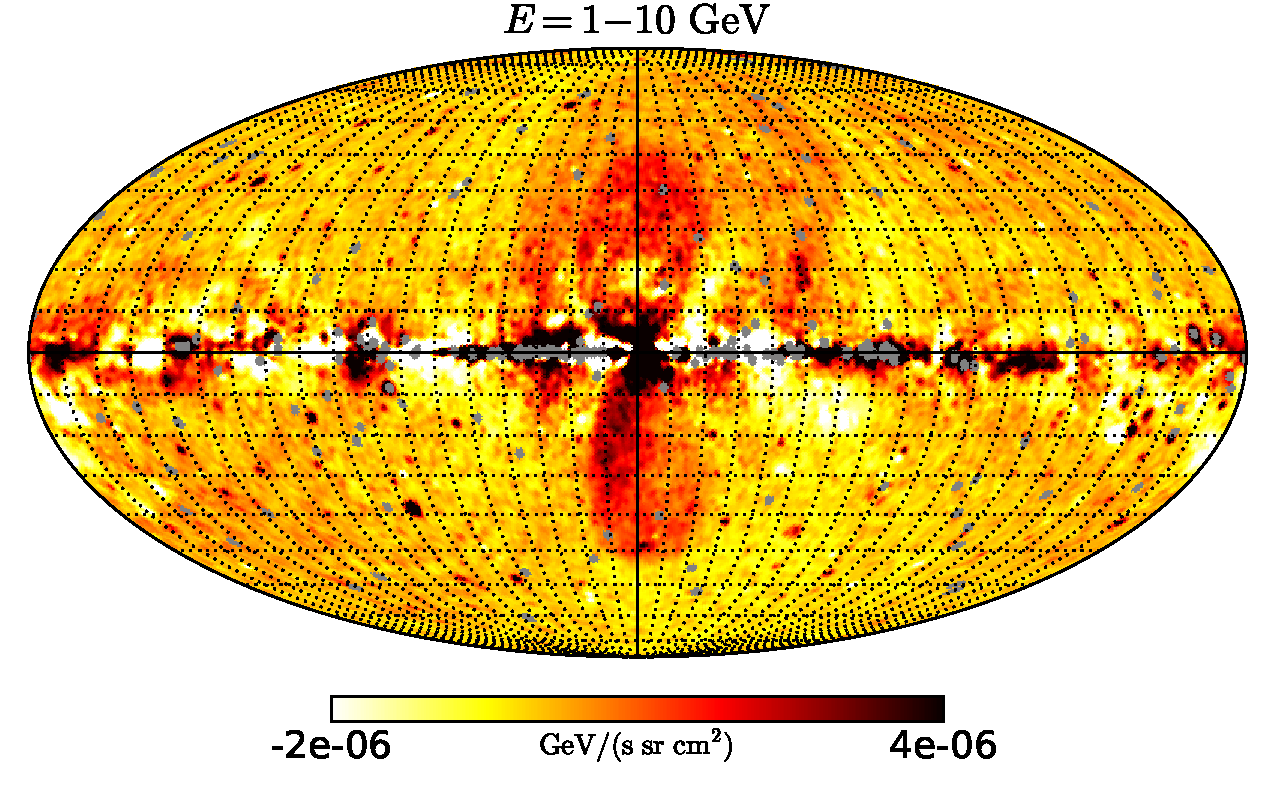
\includegraphics[width=\textwidth]{plots/Mollweide_GALPROP_source_range1.pdf}
%    	\end{subfigure} 
%    	\begin{subfigure}{0.3\textwidth}
%        	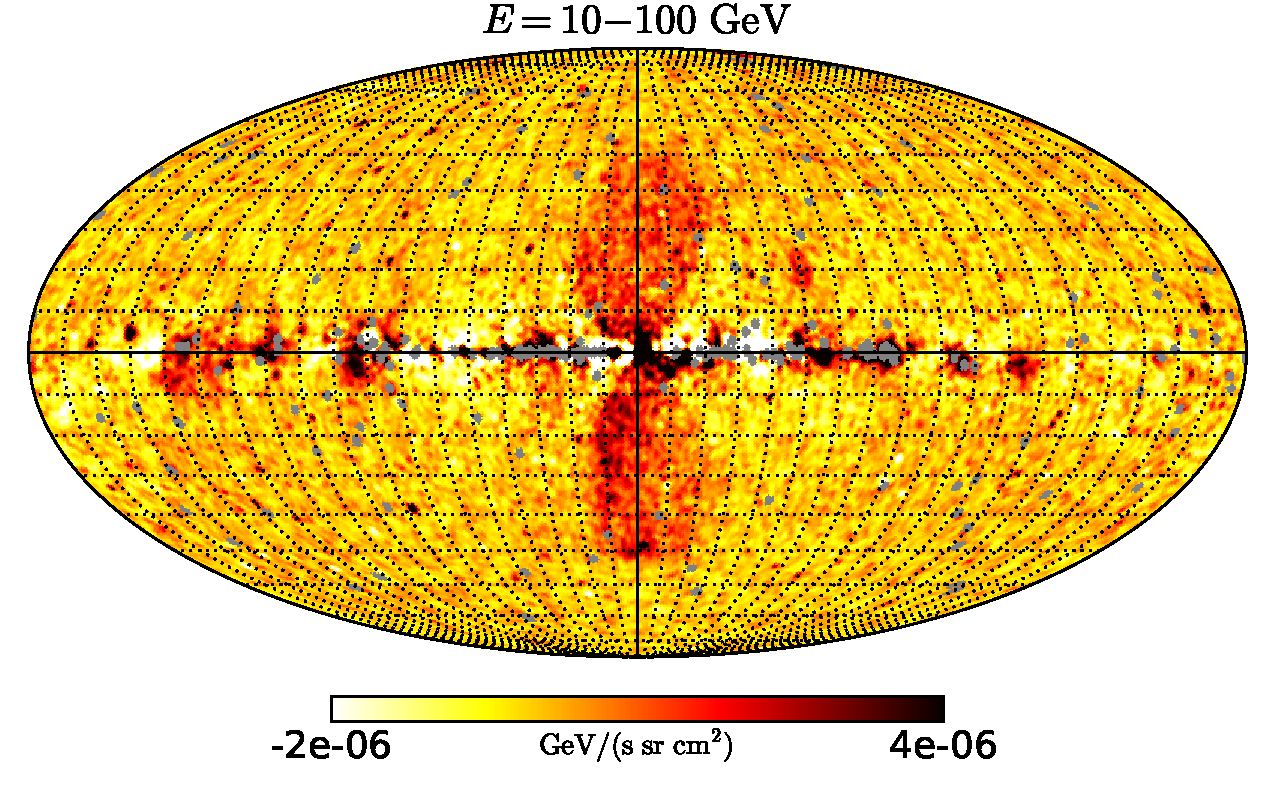
\includegraphics[width=\textwidth]{plots/Mollweide_GALPROP_source_range2.pdf}
%    	\end{subfigure}
%    	\begin{subfigure}{0.3\textwidth}
%        	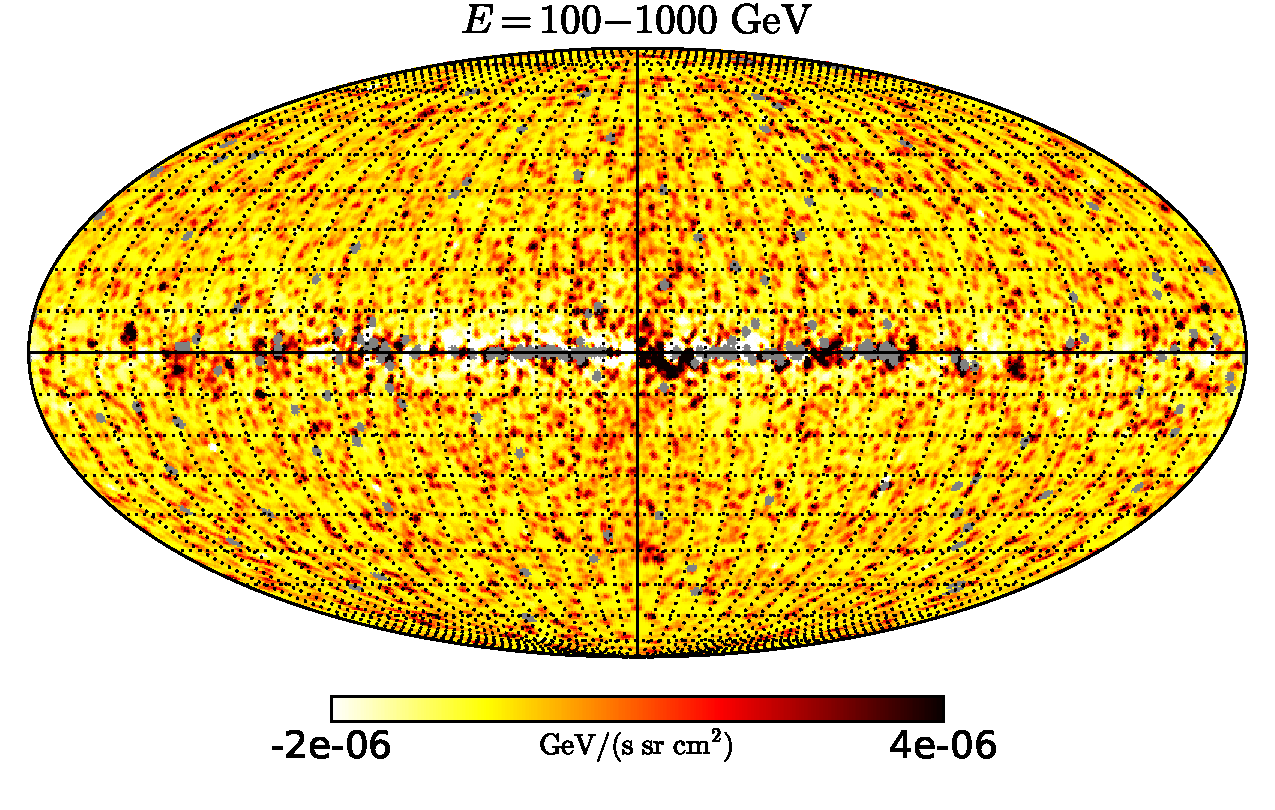
\includegraphics[width=\textwidth]{plots/Mollweide_GALPROP_source_range3.pdf}
%    	\end{subfigure}
%    	}
%  	\caption{GALPROP-model residuals in three different energy ranges.}
%  	\label{fig:Maps_GALPROP}
% \end{figure*}